% !TEX root = main.tex

%\myparagraph{Key points}
%\begin{enumerate}[1.]
%%	\item	Session $\pi$ calculus with process passing. DONE
%%	\item	Identify session $\pi$ and process passing subcalculi and their polyadic variants. DONE
%%	\item	Bisimulation theory for higher-order session semantics. DONE
%%	\item	New triggered bisimulation, related to J\&R's. DONE
%%	\item   Elementary values key to characterizations of behavioural equivalence. DONE
%	\item	Types provide techniques to prove completeness without matching. \jp{TBD}
%	\item	We are interested in encodings with properties a la Gorla. 
%                We extended them to typed setting. \jp{TBD}
%%	\item	Encode name-passing to pure process abstraction calculus, with name abstractions. DONE
%%	\item	Type of the recursion encoding uses non tail recursive type $\trec{t}{\btinp{t} \tinact}$. DONE
%%	\item	Encode higher-order semantics to first order semantics. DONE
%%	\item	Negative result. Cannot encode shared names using only shared names.
%%	\item   Extensions with higher-order abstractions and polyadicity also explored. DONE
%\end{enumerate}

%\smallskip 
%
%\myparagraph{Important things to explain}
%Explain our \HO is very small without containg name passing 
%\[ 
%\abs{x}.P \quad \appl{x}{u}
%\]

%Explain we input only characteristic processes.  
%
%\[
%\lambda x.\mapchar{S}{x}
%\]

%\subsection{Higher-Order Session Calculi}

\section{Introduction}
By combining features from the $\lambda$-calculus and the $\pi$-calculus, 
in \emph{higher-order process calculi} exchanged values may contain  processes. 
In this paper, we consider higher-order calculi with \emph{session primitives},
thus enabling the specification of reciprocal exchanges (protocols) 
for higher-order mobile processes, 
which can be verified via type-checking using \emph{session types}~\cite{honda.vasconcelos.kubo:language-primitives}.
The study of higher-order concurrency has received significant attention, 
from untyped and typed perspectives (see, e.g.,~\cite{ThomsenB:plachoasgcfhop,SangiorgiD:expmpa,San96int,JeffreyR05,MostrousY15,DBLP:journals/iandc/LanesePSS11,DBLP:conf/icalp/LanesePSS10,DBLP:conf/esop/KoutavasH11,XuActa2012}).
Although models of session-typed 
communication with features of higher-order concurrency exist~\cite{tlca07,DBLP:journals/jfp/GayV10},
their  \emph{tractable behavioural equivalences} and \emph{relative expressiveness}
remain little understood. 
Clarifying their status is not only useful for, 
e.g.,~justifying non-trivial mobile protocol
optimisations, but also for transferring key reasoning techniques
between (higher-order) session calculi. Our discovery 
is that \emph{linearity} of session types plays a vital role to 
offer new equalities and fully abstract encodability, 
which to our best knowledge have not been proposed before.   

The main higher-order language in our work, denoted \HOp,
extends the higher-order $\pi$-calculus~\cite{SangiorgiD:expmpa} with session primitives:
it contains constructs for synchronisation on shared names, 
recursion, 
name abstractions (i.e., functions from name identifiers  to processes, 
denoted $\lambda x.P$) and applications 
{(denoted $(\lambda x.P)a$)};
and session communication (value passing and
labelled choice using linear names). 
We study two significant subcalculi of \HOp, 
{which}
distil higher- and first-order mobility:
the \HO-calculus, which is \HOp without recursion and name passing, and 
the session \sessp-calculus {(here denoted~\sessp)}, which is \HOp without abstractions and applications.  
While \sessp is, 
in essence, the calculus in~\cite{honda.vasconcelos.kubo:language-primitives}, 
this paper shows that \HO  is a new core calculus 
for higher-order session concurrency.

In the first part of the paper, we address tractable behavioural equivalences
for \HOp.
A well-studied behavioural equivalence in the higher-order setting 
is \emph{context bisimilarity}~\cite{San96H},
a labelled characterisation of reduction-closed, barbed congruence, 
which offers an appropriate discriminative power at the price of heavy universal quantifications in output clauses.
Obtaining alternative characterisations 
is thus a recurring issue 
in the study of higher-order calculi. 
Our approach 
shows that protocol specifications given by session types are 
essential to  limit 
the behaviour of higher-order session processes. 
Exploiting elementary processes inhabiting session types, 
this limitation is formally enforced by 
a refined (typed) labelled transition system (LTS)
that narrows down the spectrum of allowed process behaviours, 
thus enabling tractable reasoning techniques. 
Two tractable characterisations of bisimilarity 
are then introduced. 
Remarkably, using session types we prove that these %tractable
bisimilarities coincide with context bisimilarity, without using
operators for 
name-matching.

We then move on to assess the expressivity 
 of \HOp, \HO, and \sessp as delineated by typing. 
We establish strong correspondences between 
these calculi  via type-preserving, fully abstract encodings up to 
behavioural equalities. While encoding \HOp 
into the $\pi$-calculus preserving session types 
(extending  known  results for untyped processes) is 
%{already}
significant, 
our main contribution is 
an encoding of \HOp into \HO, where name-passing is absent.  

We illustrate the essence of encoding name passing into \HO: 
to encode name output, we ``pack''
the name to be passed around into a suitable abstraction; 
upon reception, the receiver must ``unpack'' this object following a precise protocol.
More precisely, our encoding 
{of name passing}
in \HO is given as:
\begin{center}
\begin{tabular}{rcll}
  $\map{\bout{a}{b} P}$	&$=$&	$\bout{a}{ \abs{z}{\,\binp{z}{x} (\appl{x}{b})} } \map{P}$ \\
  $\map{\binp{a}{x} Q}$	&$=$&	$\binp{a}{y} \newsp{s}{\appl{y}{s} \Par \bout{\dual{s}}{\abs{x}{\map{Q}}} \inact}$
\end{tabular}
\end{center}
\noi where $a,b$ are names; $s$ and $\dual{s}$ are 
linear names (called \emph{session endpoints});
%$\lambda x.P$ is a name abstraction of $P$; $\appl{x}{a}$ is a name application; 
$\bout{a}{V} P$ and 
$\binp{a}{x} P$ denote an output and input at~$a$;   
and $\newsp{s}P$ is hiding. 
A (deterministic) reduction between   endpoints 
$s$ and $\dual{s}$ guarantees name $b$ is properly unpacked.
Encoding a recursive process $\recp{X}{P}$ is \NY{also} challenging, for 
the linearity of endpoints in $P$ must be preserved.
We encode recursion with non-tail recursive session types; for this 
we apply recent advances on the theory of session duality~\cite{TGC14,DBLP:journals/corr/abs-1202-2086}.

We further extend our encodability results to 
i)~\HOp with \emph{higher-order} abstractions (denoted \HOpp) 
and to ii)~\HOp with polyadic name passing and abstraction (\pHOp); and to
their super-calculus  (\PHOpp) (equivalent to the calculus in~\cite{tlca07}). 
A further result shows that 
shared names
%as required in the session establishment phase,
strictly add expressive power 
to session calculi. 
\figref{fig:express} summarises %our expressivity 
these results.

\begin{figure}[t]
\centering
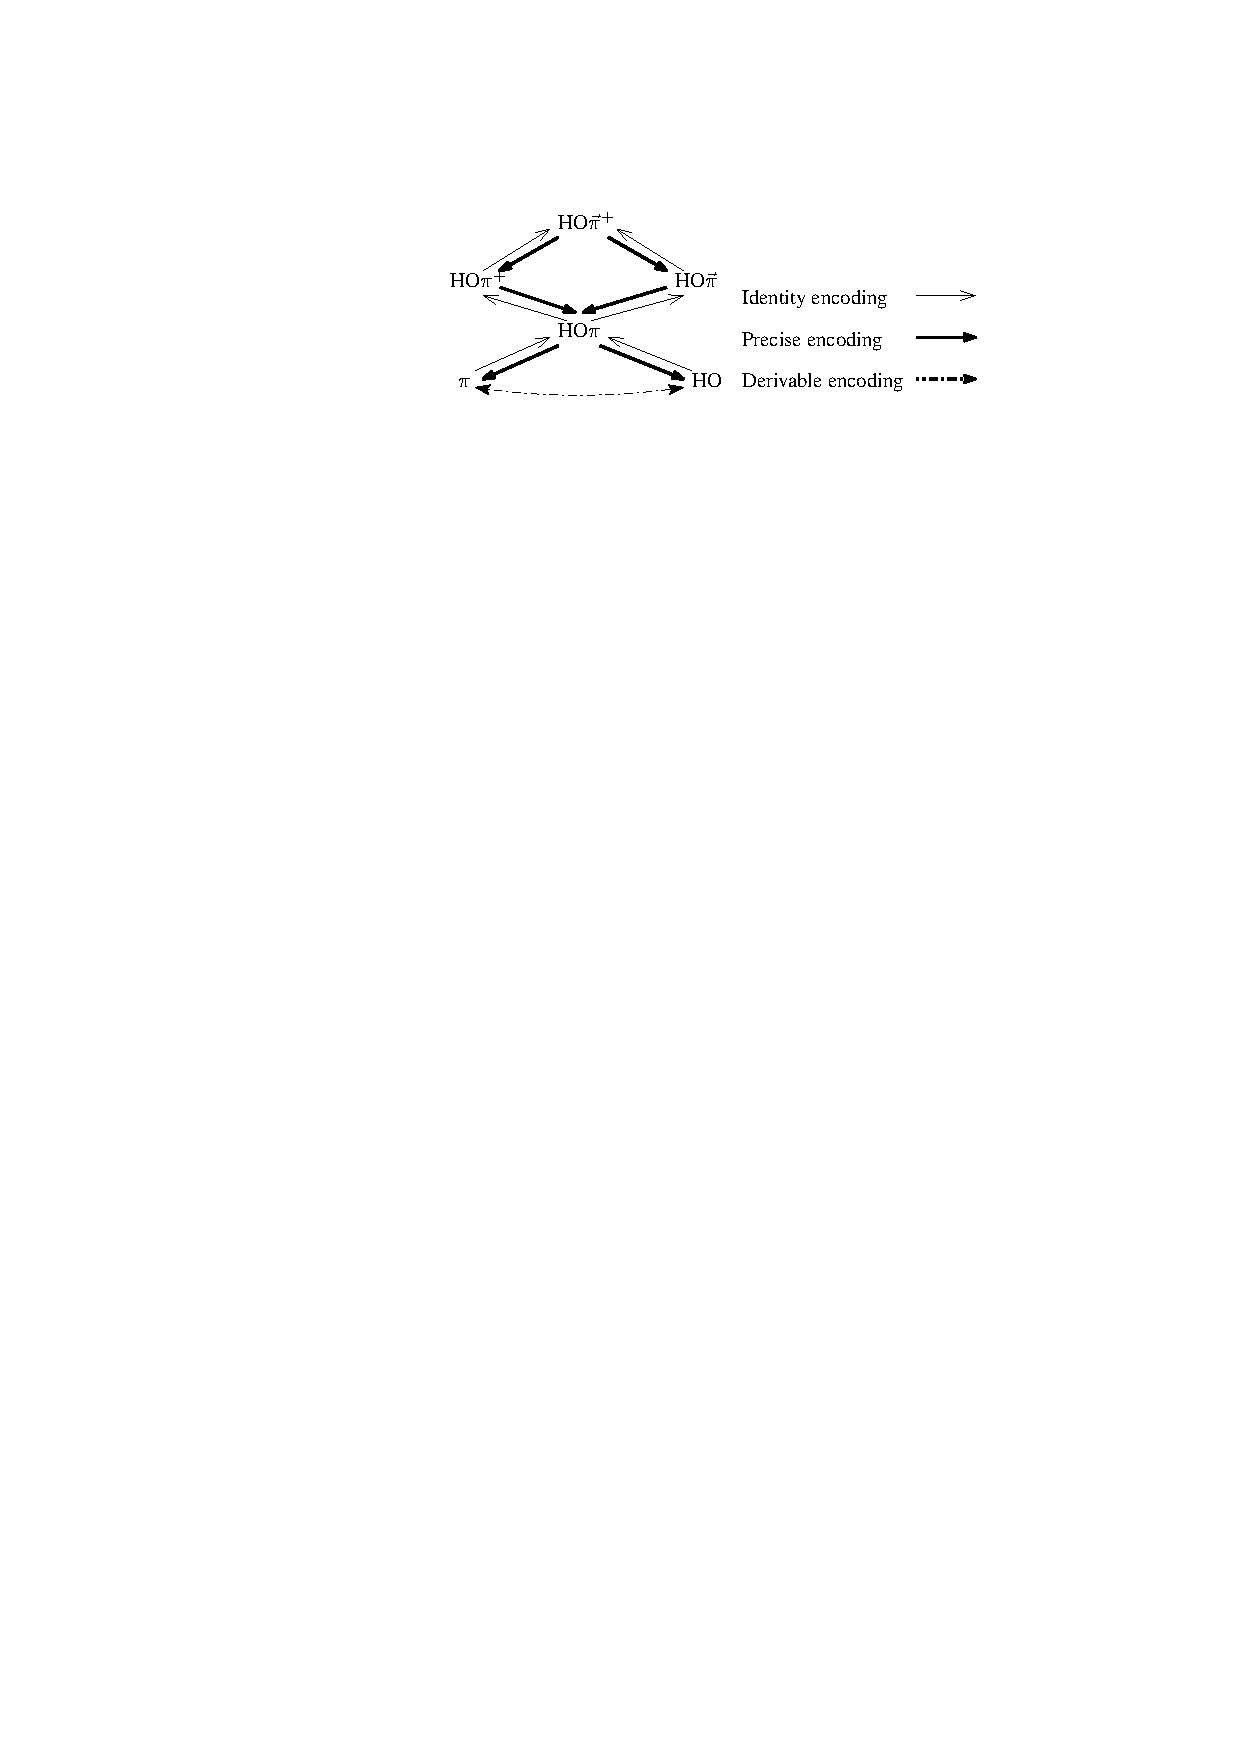
\includegraphics[scale=1]{diag.pdf}
\vspace{1mm}

	\caption{Encodability in Higher-Order Session Calculi. 
	Precise encodings are defined in \defref{def:goodenc}.
	\label{fig:express}}
\end{figure}

\smallskip

\myparagraph{Outline / Contributions.} This paper 
is structured as follows:
%
\begin{enumerate}[$\bullet$]
%	\item	\secref{sec:overview} overviews key ideas of our tractable bisimulations.

	\item	\secref{sec:calculus} presents the higher-order session calculus \HOp and its 
		subcalculi \HO and~\sessp. 

	\item	\secref{sec:types} gives the session type system
		and states type soundness for \HOp and its variants.

	\item	\secref{sec:behavioural} 
		develops \emph{higher-order} and \emph{characteristic} bisimilarities, our two
		tractable characterisations of contextual equivalence which 
		alleviate the issues of context bisimilarity~\cite{San96H}. These 
		relations are shown to coincide in \HOp (\thmref{the:coincidence}).

	\item	\secref{sec:enc} defines \emph{precise (typed) encodings} by extending encodability criteria 
		studied for
		untyped processes~(e.g.~\cite{DBLP:journals/iandc/Gorla10,DBLP:conf/icalp/LanesePSS10}).

	\item	\secref{sec:positive} and \secref{sec:negative}
		gives encodings of \HOp into \HO and of \HOp into \sessp.
		These encodings 
		are shown to be \emph{precise} (\propref{prop:prec:HOp_to_HO} and \propref{prop:prec:HOp_to_p}).
		Mutual encodings between \sessp and \HO are derivable; 
		all these calculi are thus equally expressive.
		Exploiting determinacy and typed equivalences,
		we also prove the non-encodability of shared names
		into linear names (\thmref{thm:negative}).

	\item	\secref{sec:extension} studies extensions of \HOp. We show that 
		both \HOpp (the extension with higher-order applications) 
		and \pHOp (the extension with polyadicity) are encodable in \HOp
		(\propref{prop:prec:HOpp_to_HOp} and \propref{prop:prec:pHOp_to_HOp}).
		This connects our work 
		to the existing
		higher-order session calculus in~\cite{tlca07} (here denoted  $\pHOpp$).

	\item	\secref{sec:related} concludes with related works.
The appendix collects detailed proofs of the main results.
\end{enumerate}
%\noi
%The paper is self-contained. 
%{\bf\em Additional related work, more examples, omitted definitions, and  proofs 
%can be found
%are 
%in~\cite{KouzapasPY15}.} 

